% Options for packages loaded elsewhere
\PassOptionsToPackage{unicode}{hyperref}
\PassOptionsToPackage{hyphens}{url}
%
\documentclass[
]{article}
\usepackage{amsmath,amssymb}
\usepackage{lmodern}
\usepackage{iftex}
\ifPDFTeX
  \usepackage[T1]{fontenc}
  \usepackage[utf8]{inputenc}
  \usepackage{textcomp} % provide euro and other symbols
\else % if luatex or xetex
  \usepackage{unicode-math}
  \defaultfontfeatures{Scale=MatchLowercase}
  \defaultfontfeatures[\rmfamily]{Ligatures=TeX,Scale=1}
\fi
% Use upquote if available, for straight quotes in verbatim environments
\IfFileExists{upquote.sty}{\usepackage{upquote}}{}
\IfFileExists{microtype.sty}{% use microtype if available
  \usepackage[]{microtype}
  \UseMicrotypeSet[protrusion]{basicmath} % disable protrusion for tt fonts
}{}
\makeatletter
\@ifundefined{KOMAClassName}{% if non-KOMA class
  \IfFileExists{parskip.sty}{%
    \usepackage{parskip}
  }{% else
    \setlength{\parindent}{0pt}
    \setlength{\parskip}{6pt plus 2pt minus 1pt}}
}{% if KOMA class
  \KOMAoptions{parskip=half}}
\makeatother
\usepackage{xcolor}
\usepackage[margin=1in]{geometry}
\usepackage{graphicx}
\makeatletter
\def\maxwidth{\ifdim\Gin@nat@width>\linewidth\linewidth\else\Gin@nat@width\fi}
\def\maxheight{\ifdim\Gin@nat@height>\textheight\textheight\else\Gin@nat@height\fi}
\makeatother
% Scale images if necessary, so that they will not overflow the page
% margins by default, and it is still possible to overwrite the defaults
% using explicit options in \includegraphics[width, height, ...]{}
\setkeys{Gin}{width=\maxwidth,height=\maxheight,keepaspectratio}
% Set default figure placement to htbp
\makeatletter
\def\fps@figure{htbp}
\makeatother
\setlength{\emergencystretch}{3em} % prevent overfull lines
\providecommand{\tightlist}{%
  \setlength{\itemsep}{0pt}\setlength{\parskip}{0pt}}
\setcounter{secnumdepth}{-\maxdimen} % remove section numbering
\ifLuaTeX
  \usepackage{selnolig}  % disable illegal ligatures
\fi
\IfFileExists{bookmark.sty}{\usepackage{bookmark}}{\usepackage{hyperref}}
\IfFileExists{xurl.sty}{\usepackage{xurl}}{} % add URL line breaks if available
\urlstyle{same} % disable monospaced font for URLs
\hypersetup{
  pdftitle={Assignment 1 Spatial Epidemiology},
  pdfauthor={Ferrara Lorenzo, Lucchini Marco},
  hidelinks,
  pdfcreator={LaTeX via pandoc}}

\title{Assignment 1 Spatial Epidemiology}
\usepackage{etoolbox}
\makeatletter
\providecommand{\subtitle}[1]{% add subtitle to \maketitle
  \apptocmd{\@title}{\par {\large #1 \par}}{}{}
}
\makeatother
\subtitle{Elevation of a small islet in Delta d'Ebre}
\author{Ferrara Lorenzo, Lucchini Marco}
\date{25-10-2022}

\begin{document}
\maketitle

\hypertarget{description}{%
\section{Description}\label{description}}

The data were collected during a study of the settlement pattern of
common terns on a small islet in the Delta d'Ebre (Hernandez and Ruiz,
range3), particularly in the mouths of the Ebre river. The islet was
inspected at two-day intervals throughout the range0 breeding season.
The data include the location of each nest, its elevation above sea
level, and elevations at a number of additional points (points without
nest) on the islet. In the file called elevationsIslet.txt, contains the
information of the coordinates and elevation above sea, and in file,
called poly84.txt contains the coordinates of the borders of the islet.
The aim is to predict the elevation above sea level along the small
islet using a kriging interpolation.

\hypertarget{explore-the-requirement-of-stationary-mean-of-the-process.-in-case-this-requirement-is-not-met-detrend-the-data-to-ensure-that-the-process-is-stationary-in-mean.-discuss-the-results-and-show-the-plot-of-the-results}{%
\subsection{1) Explore the requirement of stationary mean of the
process. In case this requirement is not met, detrend the data to ensure
that the process is stationary in mean. Discuss the results and show the
plot of the
results}\label{explore-the-requirement-of-stationary-mean-of-the-process.-in-case-this-requirement-is-not-met-detrend-the-data-to-ensure-that-the-process-is-stationary-in-mean.-discuss-the-results-and-show-the-plot-of-the-results}}

Firstly, we plot the locations to see the spatial distribution of the
data

\begin{center}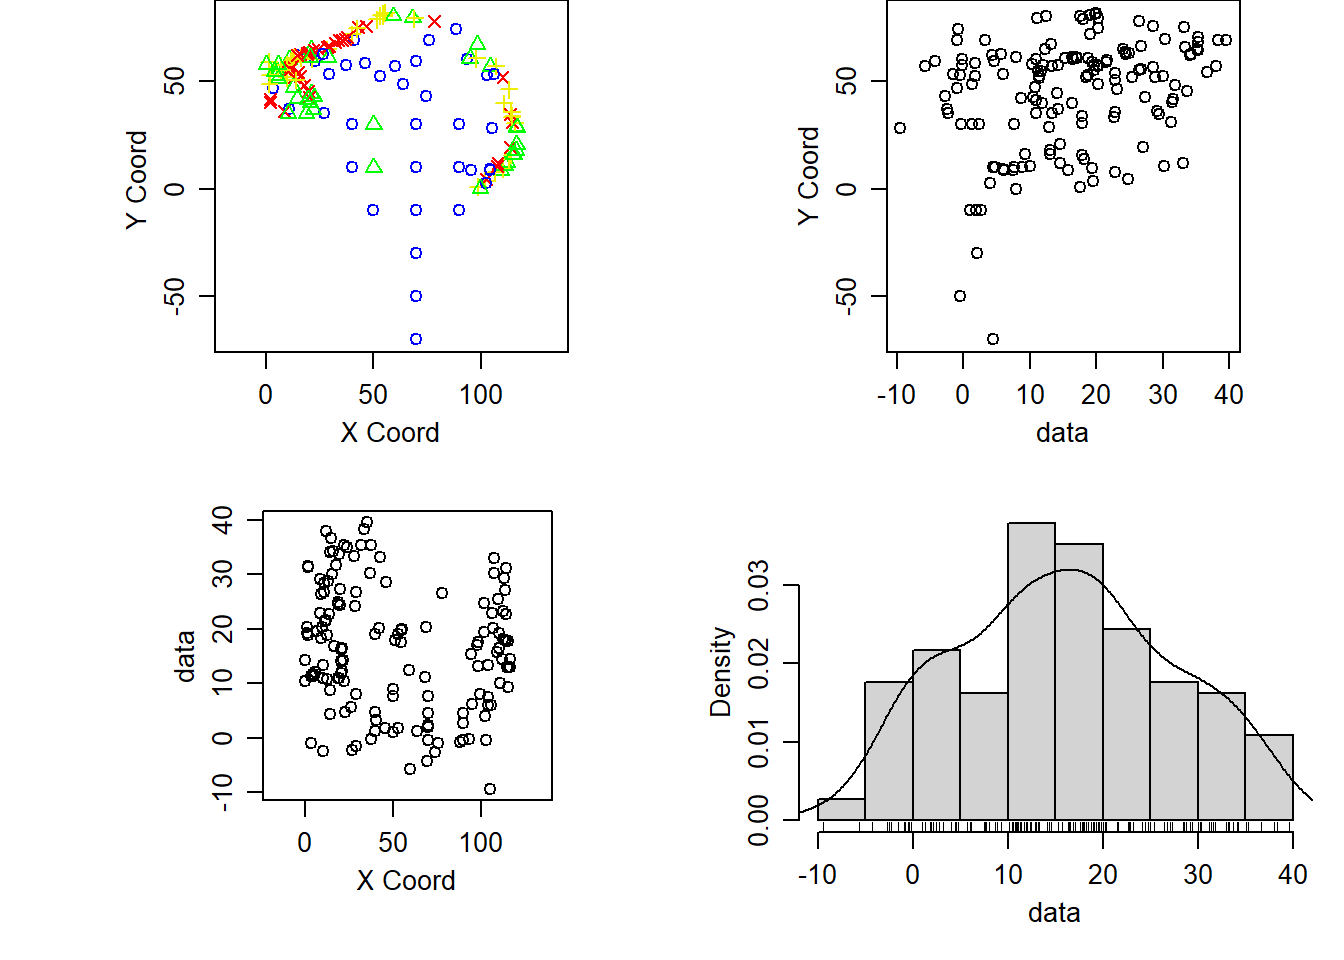
\includegraphics[width=0.7\linewidth]{Assignment_1_FINALE_files/figure-latex/unnamed-chunk-5-1} \end{center}

We also look at the distribution in relation to the x-coordinates (E-W)
and y-coordinates(N-S).

\begin{center}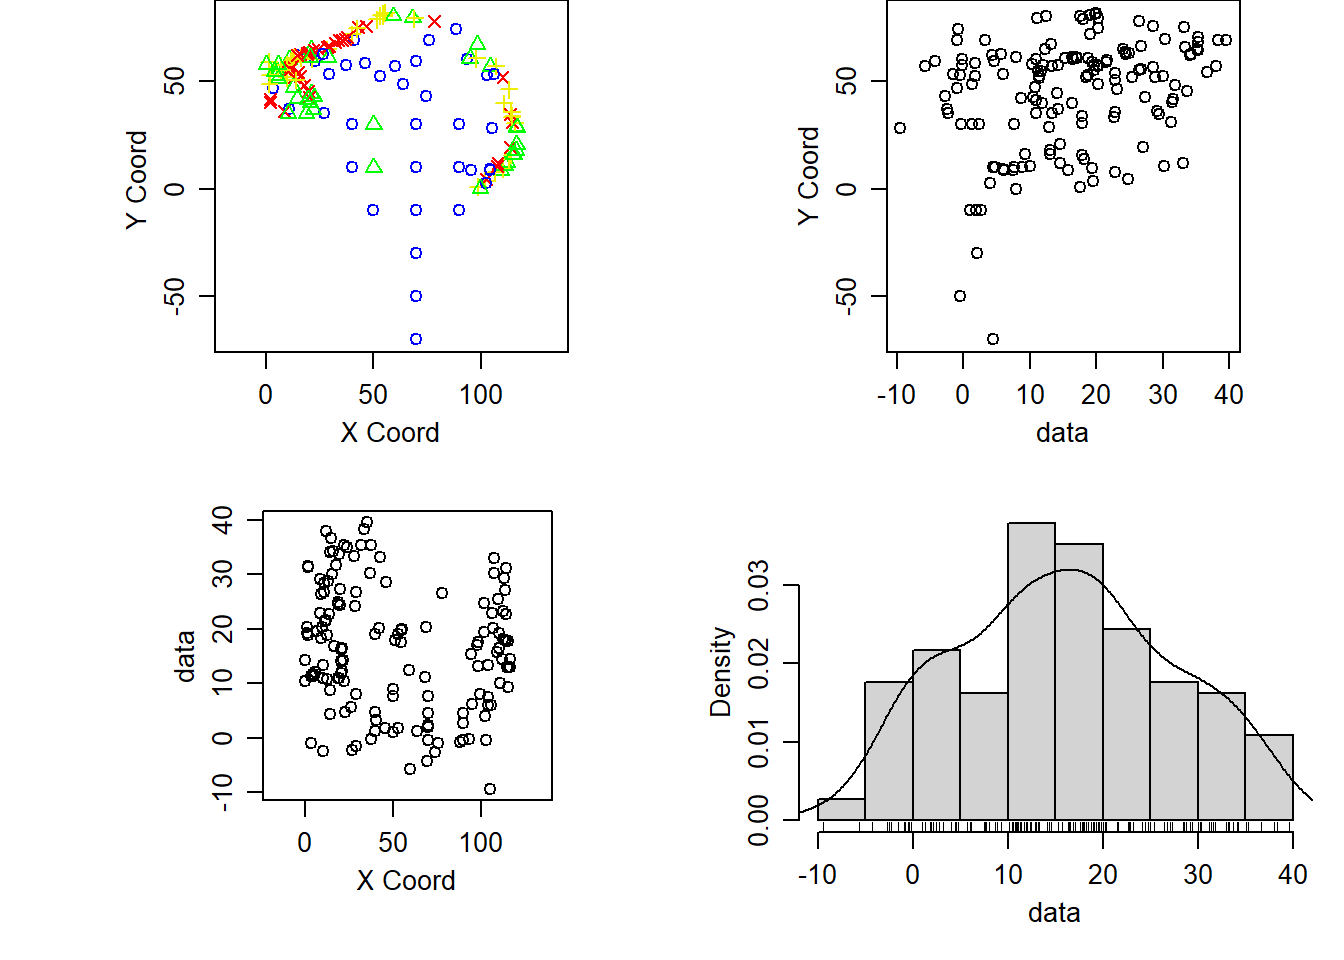
\includegraphics[width=0.7\linewidth]{Assignment_1_FINALE_files/figure-latex/unnamed-chunk-6-1} \end{center}

The plots show a concentration of high values in the extreme east and
west of the islet and we can observe a greater density in the north.

The process doesn't seem stationary, indeed there is a clear quadratic
trend along the x direction. In addition we try using the y direction as
regressor, to find a possible linear or quadratic trend.

\begin{verbatim}
## 
## Call:
## lm(formula = data ~ x + y + I(x^2) + I(y^2), data = dataset)
## 
## Residuals:
##     Min      1Q  Median      3Q     Max 
## -22.639  -6.417  -0.964   6.024  22.744 
## 
## Coefficients:
##               Estimate Std. Error t value Pr(>|t|)    
## (Intercept) 17.4502678  2.8429177   6.138 7.78e-09 ***
## x           -0.4938096  0.1103379  -4.475 1.55e-05 ***
## y            0.0349038  0.0570014   0.612    0.541    
## I(x^2)       0.0040706  0.0009267   4.393 2.17e-05 ***
## I(y^2)       0.0019508  0.0008841   2.206    0.029 *  
## ---
## Signif. codes:  0 '***' 0.001 '**' 0.01 '*' 0.05 '.' 0.1 ' ' 1
## 
## Residual standard error: 10.19 on 143 degrees of freedom
## Multiple R-squared:  0.2026, Adjusted R-squared:  0.1803 
## F-statistic: 9.082 on 4 and 143 DF,  p-value: 1.446e-06
\end{verbatim}

The linear term in y doesn't seem significant, so we remove it.

\begin{verbatim}
## 
## Call:
## lm(formula = data ~ x + I(x^2) + I(y^2), data = dataset)
## 
## Residuals:
##     Min      1Q  Median      3Q     Max 
## -22.768  -6.656  -1.081   6.166  22.879 
## 
## Coefficients:
##               Estimate Std. Error t value Pr(>|t|)    
## (Intercept) 18.3842839  2.3938539   7.680 2.23e-12 ***
## x           -0.5192823  0.1019735  -5.092 1.09e-06 ***
## I(x^2)       0.0042621  0.0008705   4.896 2.59e-06 ***
## I(y^2)       0.0023697  0.0005587   4.241 3.96e-05 ***
## ---
## Signif. codes:  0 '***' 0.001 '**' 0.01 '*' 0.05 '.' 0.1 ' ' 1
## 
## Residual standard error: 10.17 on 144 degrees of freedom
## Multiple R-squared:  0.2005, Adjusted R-squared:  0.1838 
## F-statistic: 12.04 on 3 and 144 DF,  p-value: 4.456e-07
\end{verbatim}

Now we have obtained a model in which all regressors seem to be
significant. We save the residuals of our linear model and look at the
de-trended data:

What we now obtain is a more homogeneous distribution of the data around
the value 0.

\begin{center}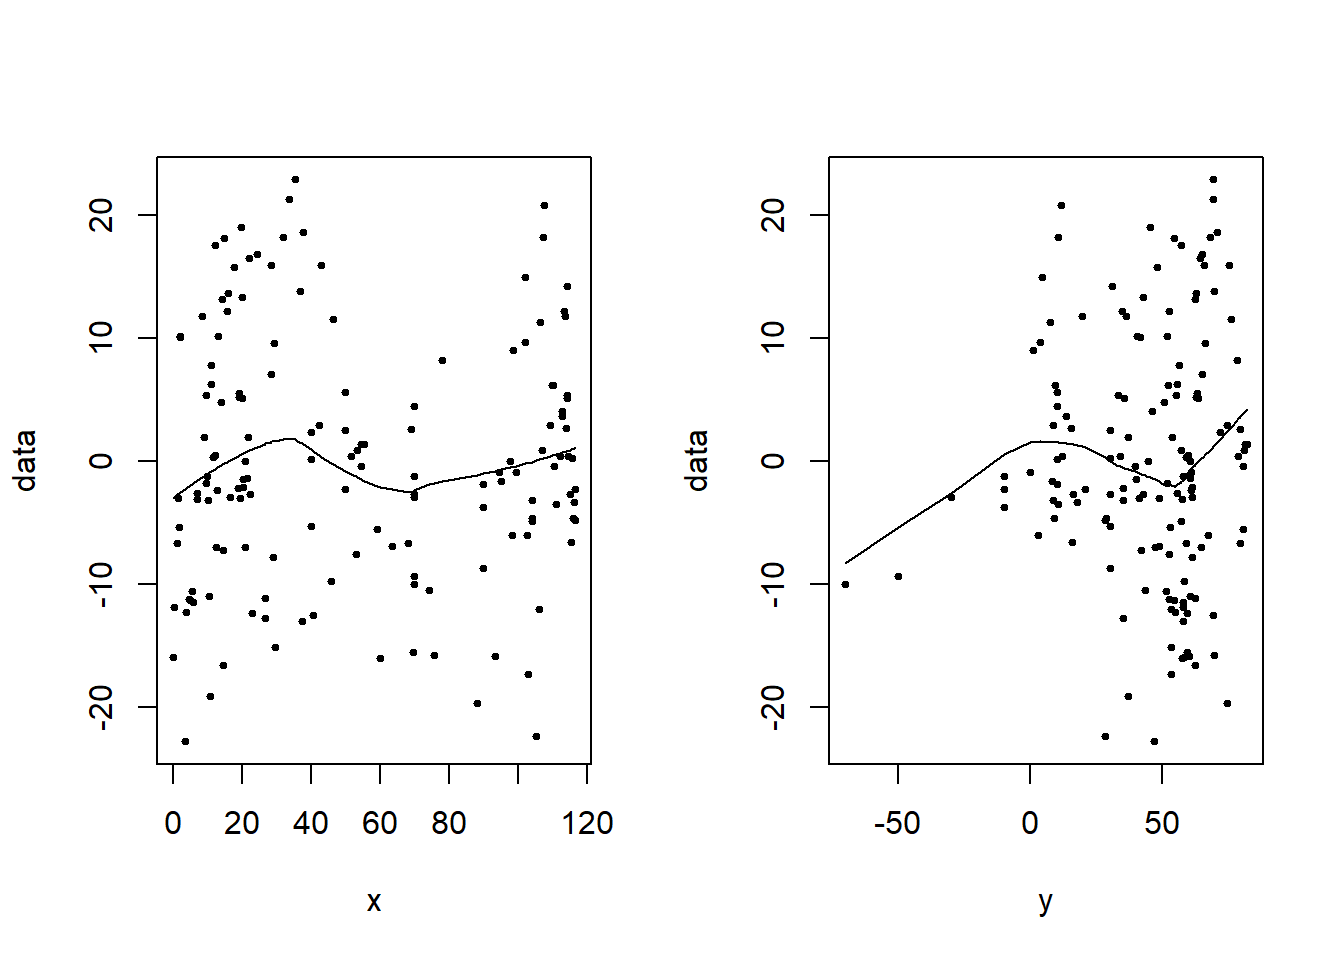
\includegraphics[width=0.7\linewidth]{Assignment_1_FINALE_files/figure-latex/unnamed-chunk-12-1} \end{center}

We don't notice any particular trend so this new dataset seems
stationary!

\newpage

\hypertarget{explore-the-spatial-dependence-of-the-elevation-variable-using-the-variogram-cloud-and-bins-and-the-empirical-variogram.-discuss-the-results-and-plot-them}{%
\subsection{2) Explore the spatial dependence of the elevation variable
using the variogram cloud and bins and the empirical variogram. Discuss
the results and plot
them}\label{explore-the-spatial-dependence-of-the-elevation-variable-using-the-variogram-cloud-and-bins-and-the-empirical-variogram.-discuss-the-results-and-plot-them}}

We try to analyse the spatial dependence through a Variogram Cloud,
using the Robust Estimators (since the classical one might consider
outliers those values which are not necessarily outliers)

\begin{center}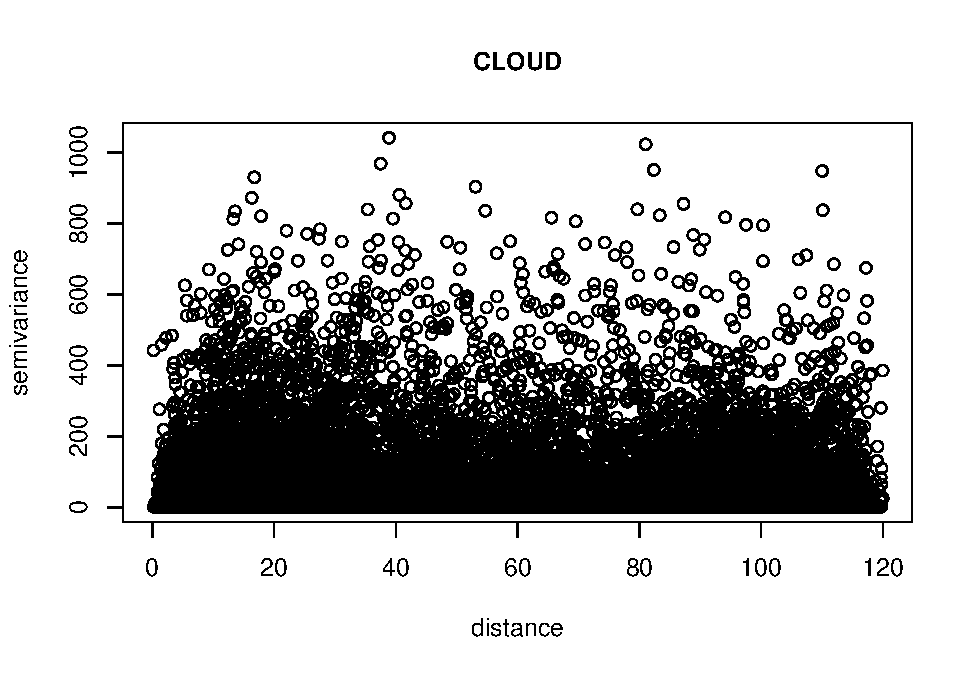
\includegraphics[width=0.7\linewidth]{Assignment_1_FINALE_files/figure-latex/unnamed-chunk-13-1} \end{center}

The variability at small distances appears a bit greater than that for
larger distances. =\textgreater{} We reduce the density of the plot by
reducing the maximum distance over which the variance are calculate.

\begin{center}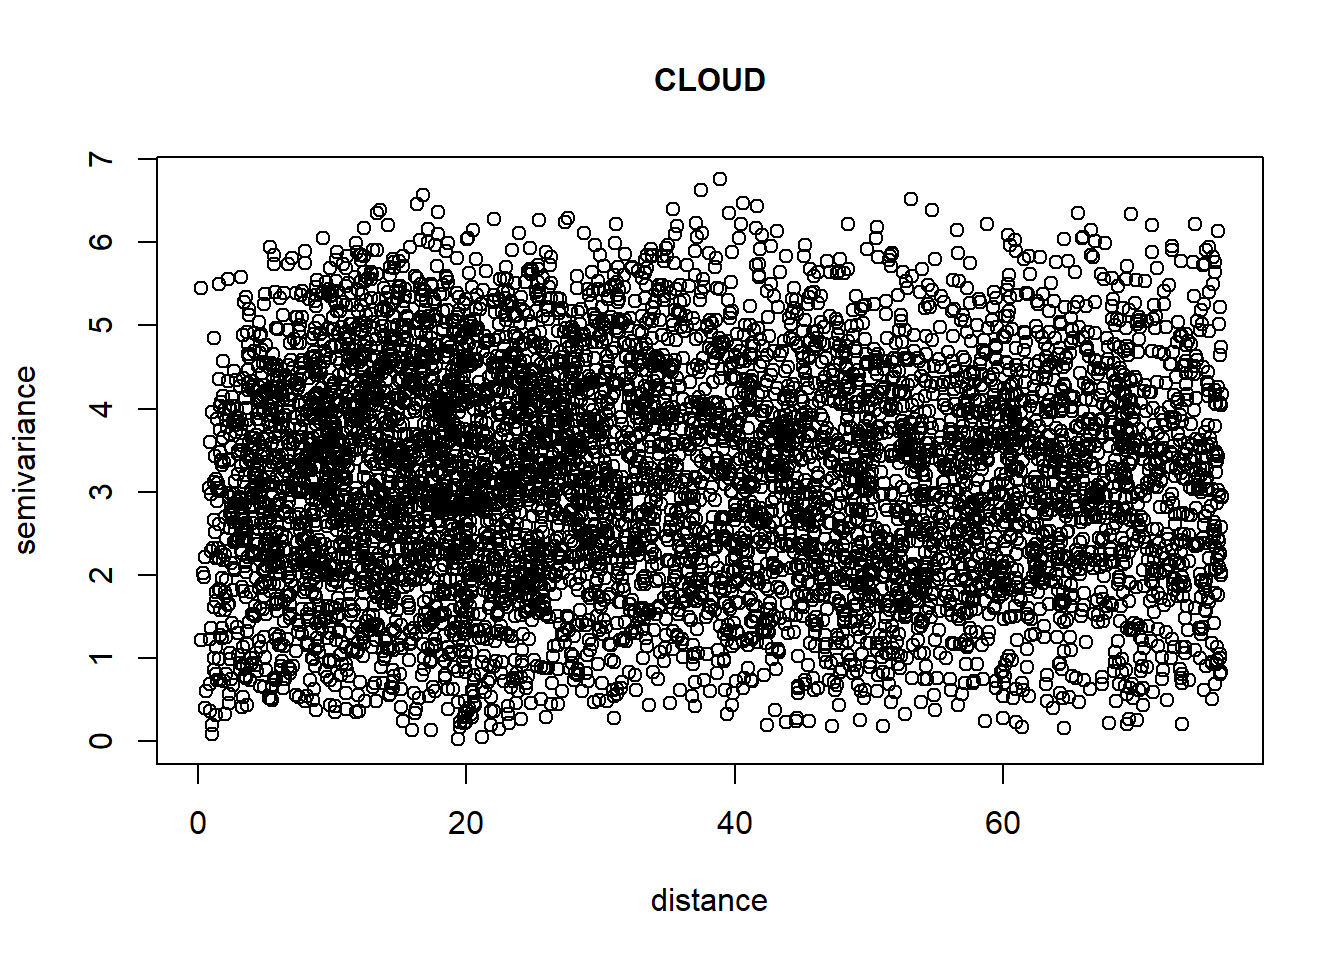
\includegraphics[width=0.7\linewidth]{Assignment_1_FINALE_files/figure-latex/unnamed-chunk-14-1} \end{center}

\begin{center}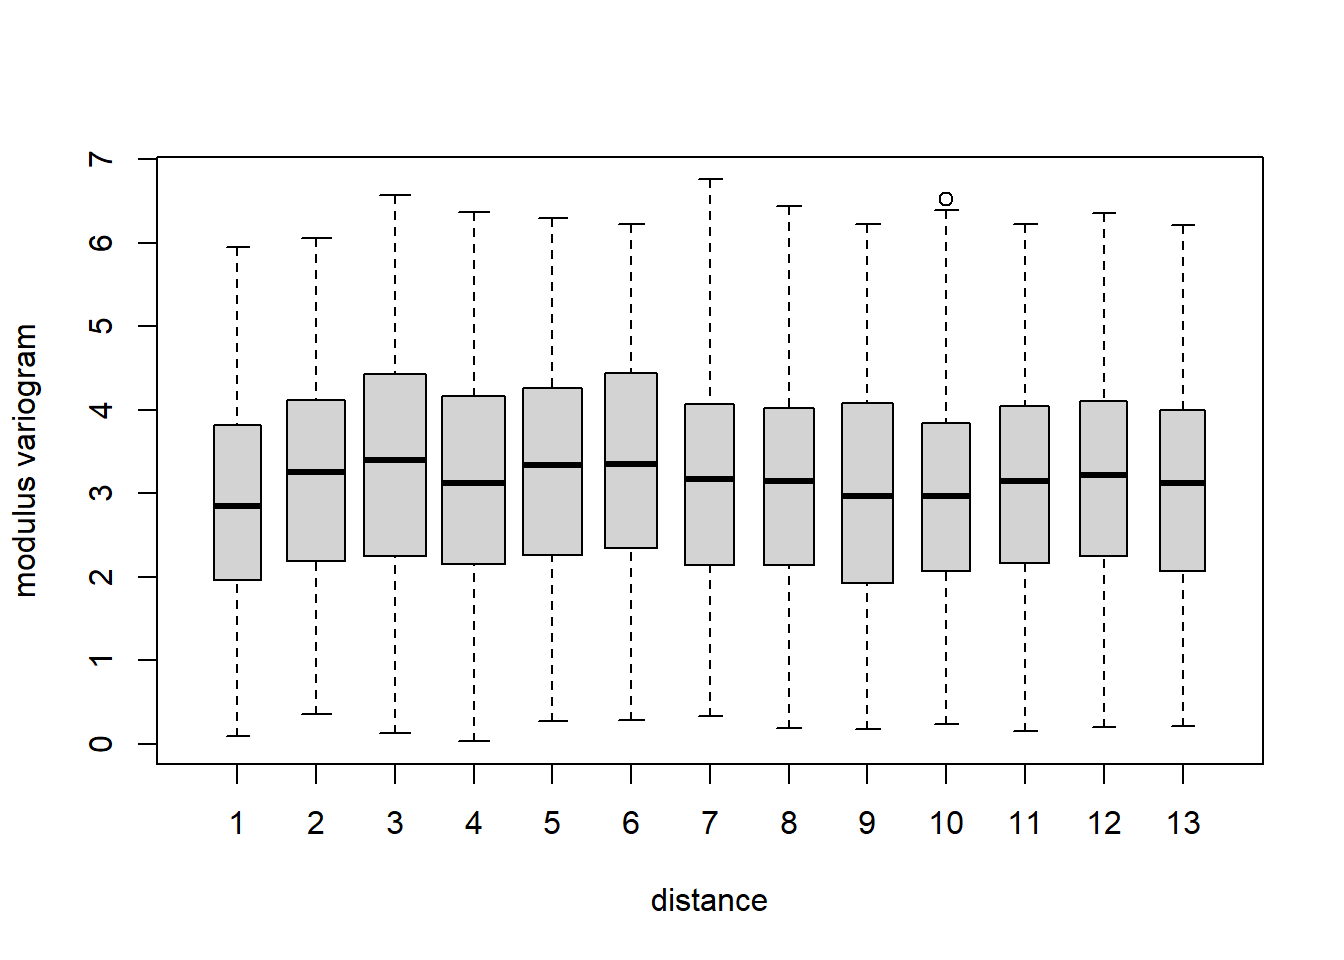
\includegraphics[width=0.7\linewidth]{Assignment_1_FINALE_files/figure-latex/unnamed-chunk-15-1} \end{center}

=\textgreater{} All the bins have at least pairs.min=30 observations
each, indeed they have:

Empirical Variogram

\begin{center}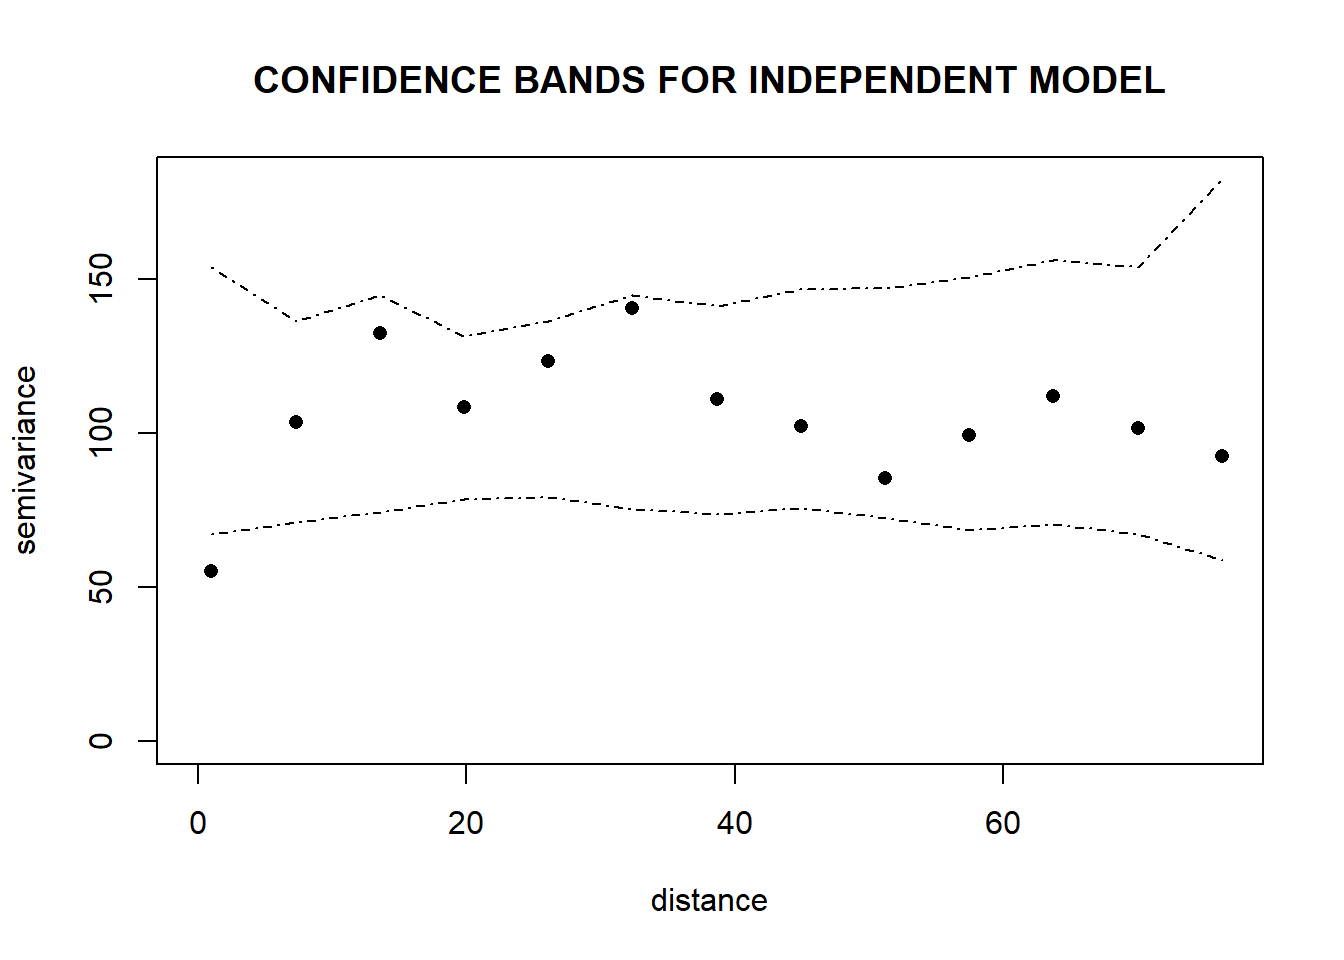
\includegraphics[width=0.7\linewidth]{Assignment_1_FINALE_files/figure-latex/unnamed-chunk-20-1} \end{center}

In the variogram of the residuals the values increases until certain
distance, and then they keep constant. That's ok since it's the
behaviour that we expect from a stationary variogram.

\newpage

\hypertarget{check-the-hypothesis-of-the-spatial-independence}{%
\subsection{3) Check the hypothesis of the spatial
independence}\label{check-the-hypothesis-of-the-spatial-independence}}

To check the hypothesis of the spatial independence we use a Monte Carlo
approach

\begin{verbatim}
## variog.env: generating 3000 simulations by permutating data values
## variog.env: computing the empirical variogram for the 3000 simulations
## variog.env: computing the envelops
\end{verbatim}

\begin{center}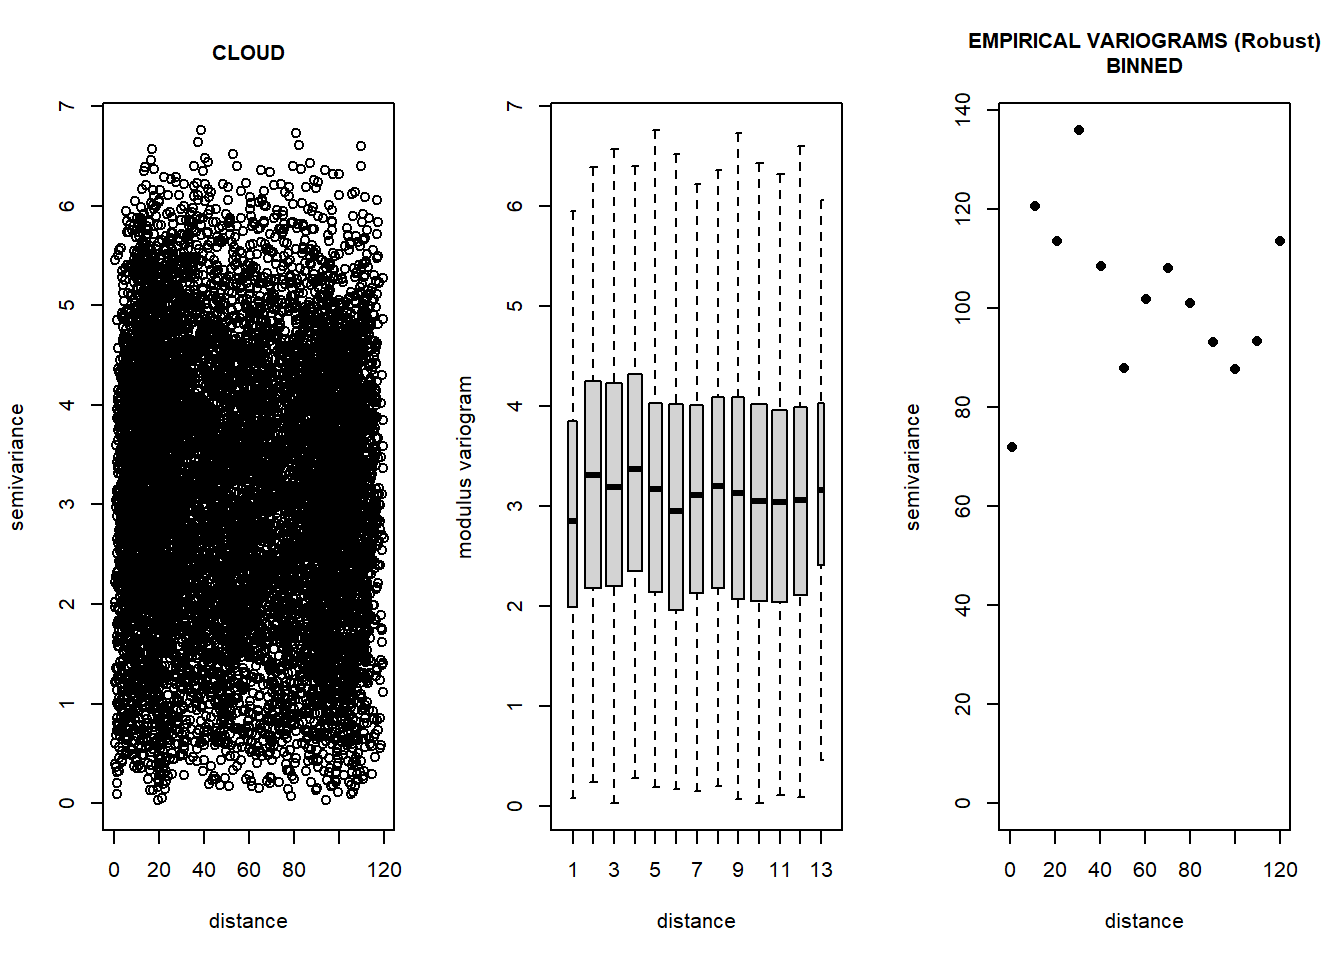
\includegraphics[width=0.7\linewidth]{Assignment_1_FINALE_files/figure-latex/unnamed-chunk-22-1} \end{center}

All the values of the empirical variogram are inside the envelope,
therefore the process has no spatial dependence.

\newpage

\hypertarget{check-the-isotropy-property-of-the-process.-comment-the-results-its-not-necessary-to-overcome-the-anisotropy.}{%
\subsection{4) Check the isotropy property of the process. Comment the
results, it's not necessary to overcome the
anisotropy.}\label{check-the-isotropy-property-of-the-process.-comment-the-results-its-not-necessary-to-overcome-the-anisotropy.}}

To check the anisotropy we need to compute the directional variogram in
the 4 main directions: 0º, 45º,90º and 135º.

\begin{center}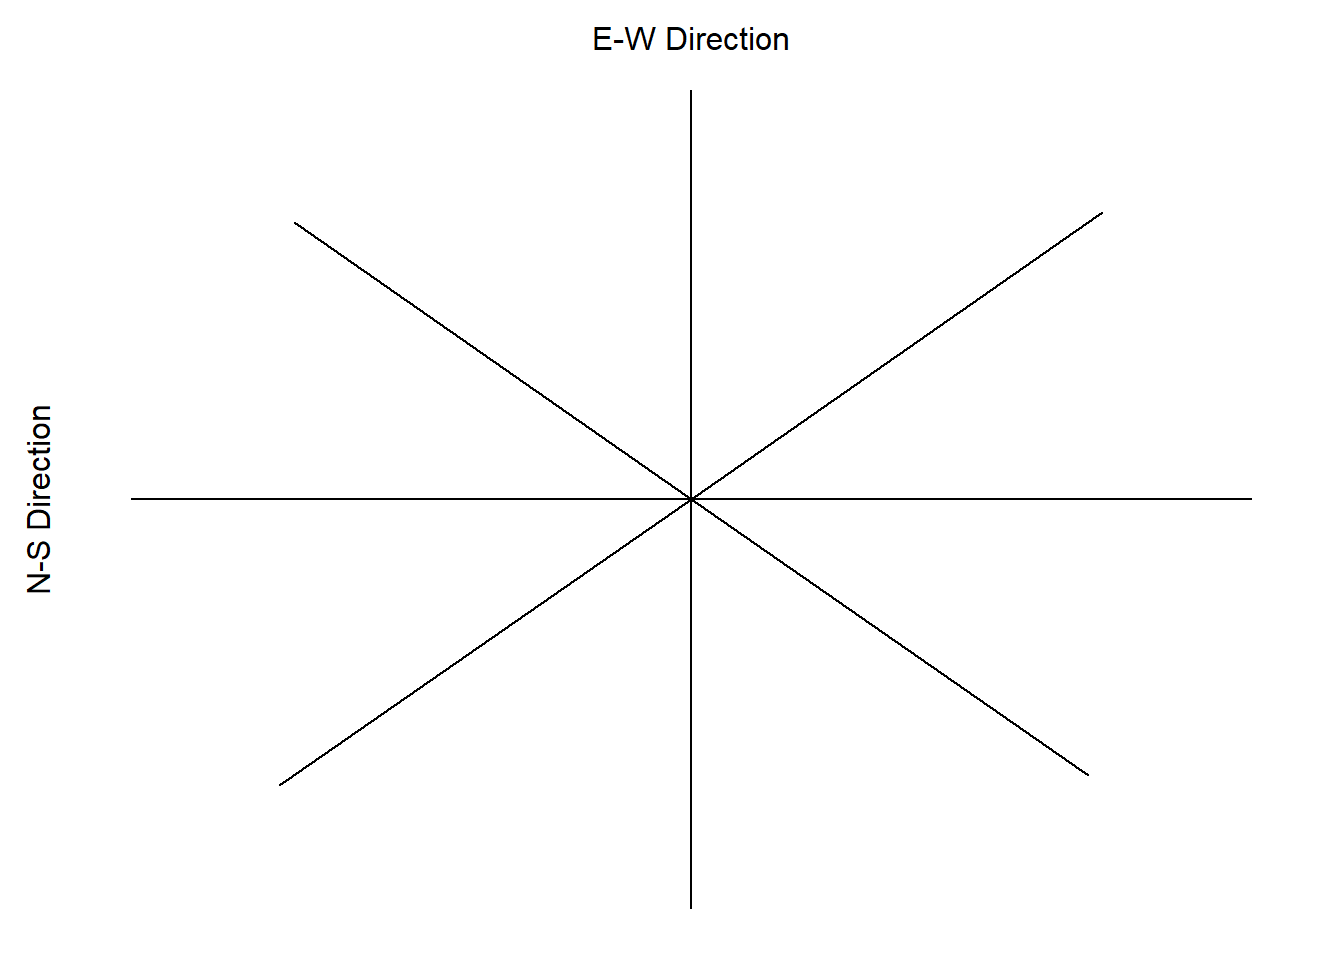
\includegraphics[width=0.7\linewidth]{Assignment_1_FINALE_files/figure-latex/unnamed-chunk-24-1} \end{center}

The directional variograms don't seem to be perfectly overlapping: they
might have the a different sill, in particular the variogram seems to
have a higher value along the 90° direction =\textgreater{} Geometrical
anistropy

Let's also analyse the range observing the Rose Diagram:

\begin{center}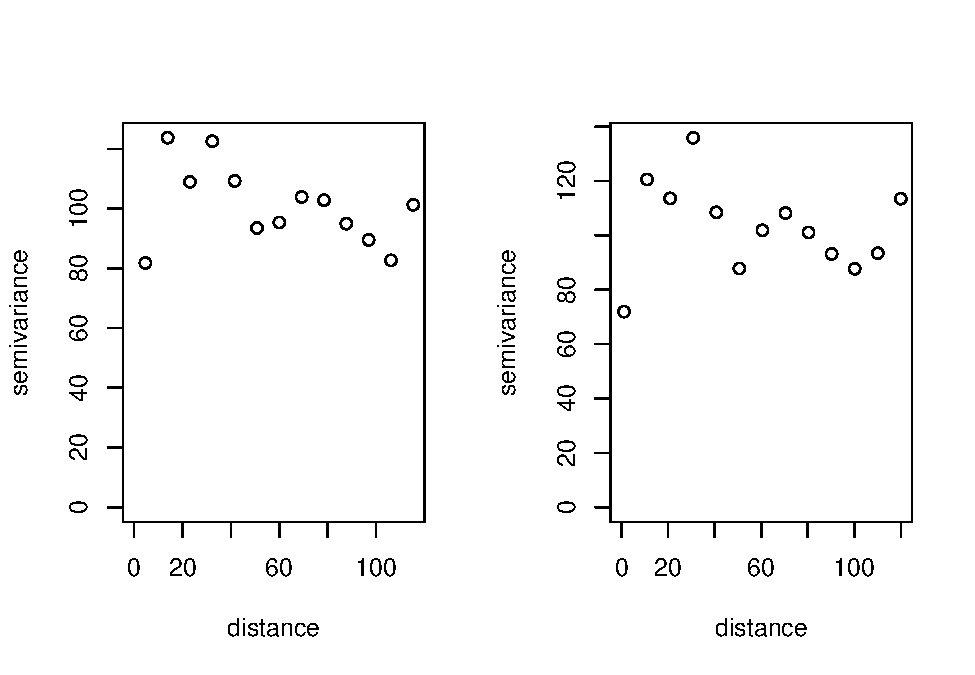
\includegraphics[width=0.7\linewidth]{Assignment_1_FINALE_files/figure-latex/unnamed-chunk-25-1} \end{center}

We can observe that the Rose diagram is more or less a circle. At
different directions, the variance is reached more or less at the same
range. Then, this process is isotropic.

OPPURE

We notice that the Rose diagram is not perfectly circular: it is
slightly elliptical, with major range in the 45 direction
=\textgreater{} Zonal anistropy.

=\textgreater{} In conclusion we have a combined anisotropy, so we can't
make the assumption of isotropic process, which is necessary for the
correct use of the kriging techniques, since the theoretical variograms
used for krigring are based on isotropic models.

\newpage

\hypertarget{propose-four-theoretical-variograms-and-estimate-the-parameters-via-restricted-maximum-likelihood-or-weighed-least-square.-select-the-two-variograms-which-best-fit-the-data.-explain-the-parameters-of-the-chosen-variogram-sill-nugget-range-and-kappa.}{%
\subsection{5) Propose four theoretical variograms and estimate the
parameters via restricted maximum likelihood or weighed least square.
Select the two variograms which best fit the data. Explain the
parameters of the chosen variogram (sill, nugget, range and
kappa).}\label{propose-four-theoretical-variograms-and-estimate-the-parameters-via-restricted-maximum-likelihood-or-weighed-least-square.-select-the-two-variograms-which-best-fit-the-data.-explain-the-parameters-of-the-chosen-variogram-sill-nugget-range-and-kappa.}}

We'll use a Maximum Likelihood approach

\hypertarget{exponential}{%
\subsubsection{Exponential}\label{exponential}}

\begin{verbatim}
## likfit: estimated model parameters:
##     beta    tausq  sigmasq      phi 
## "-2.631" "34.598" "71.657" " 6.083" 
## Practical Range with cor=0.05 for asymptotic range: 18.2225
## 
## likfit: maximised log-likelihood = -531.4
\end{verbatim}

\hypertarget{gaussian}{%
\subsubsection{Gaussian}\label{gaussian}}

\begin{verbatim}
## likfit: estimated model parameters:
##     beta    tausq  sigmasq      phi 
## "-2.786" "41.157" "66.712" " 5.601" 
## Practical Range with cor=0.05 for asymptotic range: 9.693811
## 
## likfit: maximised log-likelihood = -529.8
\end{verbatim}

\hypertarget{spherical}{%
\subsubsection{Spherical}\label{spherical}}

\begin{verbatim}
## likfit: estimated model parameters:
##     beta    tausq  sigmasq      phi 
## "-2.758" "36.363" "69.395" "12.992" 
## Practical Range with cor=0.05 for asymptotic range: 12.99251
## 
## likfit: maximised log-likelihood = -530.3
\end{verbatim}

\hypertarget{matern}{%
\subsubsection{Matern}\label{matern}}

\begin{verbatim}
## likfit: estimated model parameters:
##      beta     tausq   sigmasq       phi     kappa 
## "-2.7802" "40.9994" "66.7522" " 0.5757" "24.1330" 
## Practical Range with cor=0.05 for asymptotic range: 9.889255
## 
## likfit: maximised log-likelihood = -529.8
\end{verbatim}

\begin{center}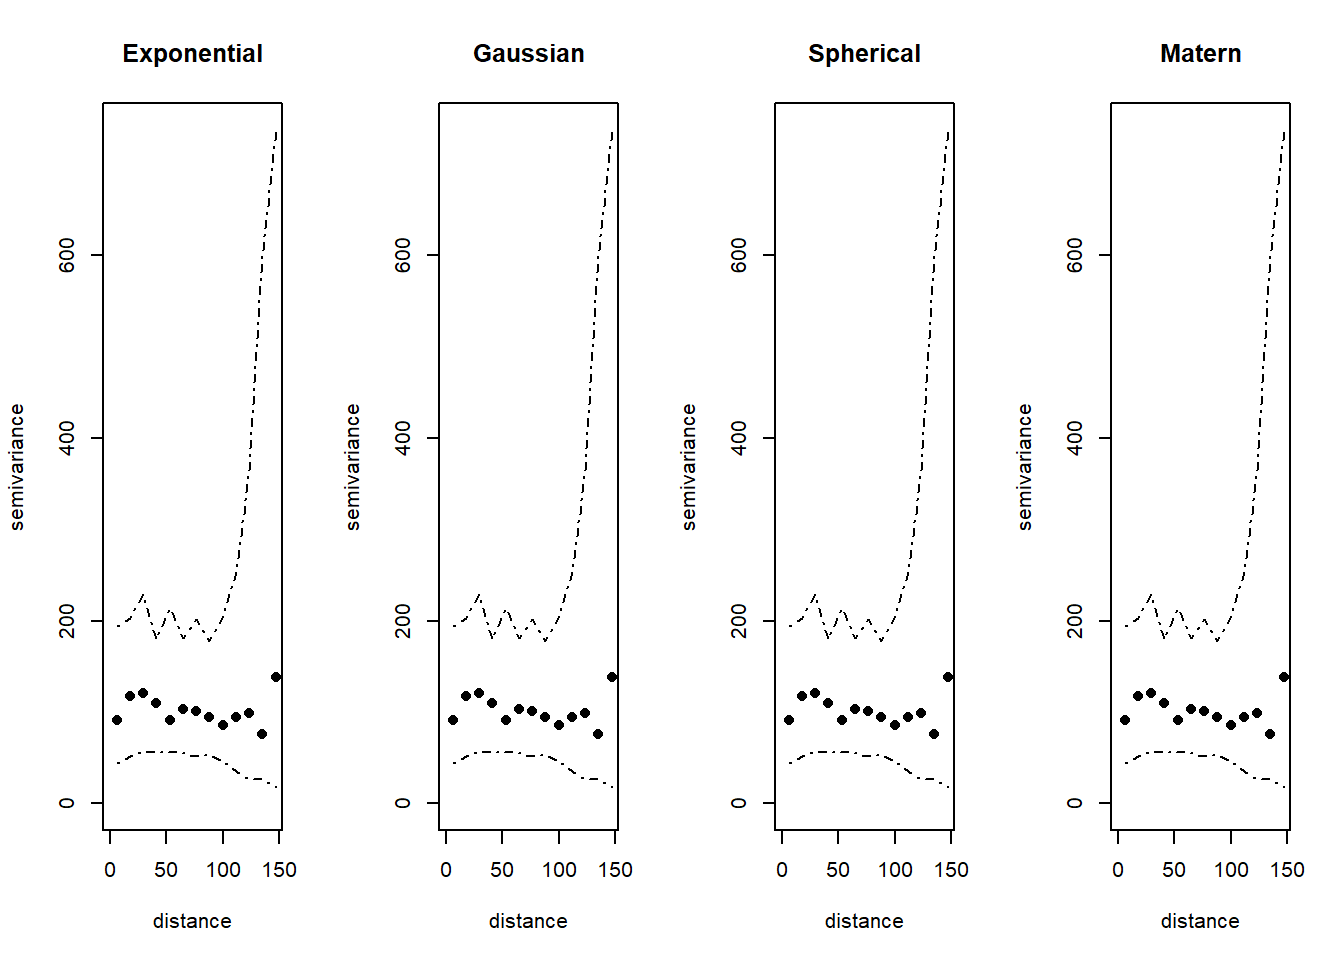
\includegraphics[width=0.7\linewidth]{Assignment_1_FINALE_files/figure-latex/unnamed-chunk-33-1} \end{center}

\begin{center}\includegraphics[width=0.7\linewidth]{Assignment_1_FINALE_files/figure-latex/unnamed-chunk-35-1} \end{center}

All the simulated variograms contain the empirical variogram so we don't
have evidence to exclude any model.

Let's compare the different models

\begin{verbatim}
##         model loglikelihood
## 4      matern     -529.7873
## 2    gaussian     -529.7890
## 3   spherical     -530.2743
## 1 exponential     -531.3895
\end{verbatim}

The two fitted models with the highest loglikelihood are the Matern
model and the Gaussian model. So we'll use these two to perform the
kriging prediction step.

\newpage

\hypertarget{predict-the-elevations-along-all-the-area-of-study-using-the-two-variogram-selected-in-point-4.-discuss-the-type-of-kriging-chosen}{%
\subsection{6) Predict the elevations along all the area of study using
the two variogram selected in point 4. Discuss the type of kriging
chosen:}\label{predict-the-elevations-along-all-the-area-of-study-using-the-two-variogram-selected-in-point-4.-discuss-the-type-of-kriging-chosen}}

\hypertarget{a.-compare-both-kriging-predictions-using-cross-validation-and-propose-the-best-model.}{%
\subsubsection{a. Compare both kriging predictions using
cross-validation, and propose the best
model.}\label{a.-compare-both-kriging-predictions-using-cross-validation-and-propose-the-best-model.}}

\hypertarget{b.-show-the-predictions-and-their-standard-errors.}{%
\subsubsection{b. Show the predictions and their standard
errors.}\label{b.-show-the-predictions-and-their-standard-errors.}}

First werate a grid where we'll perform our kriging predicitons

\begin{center}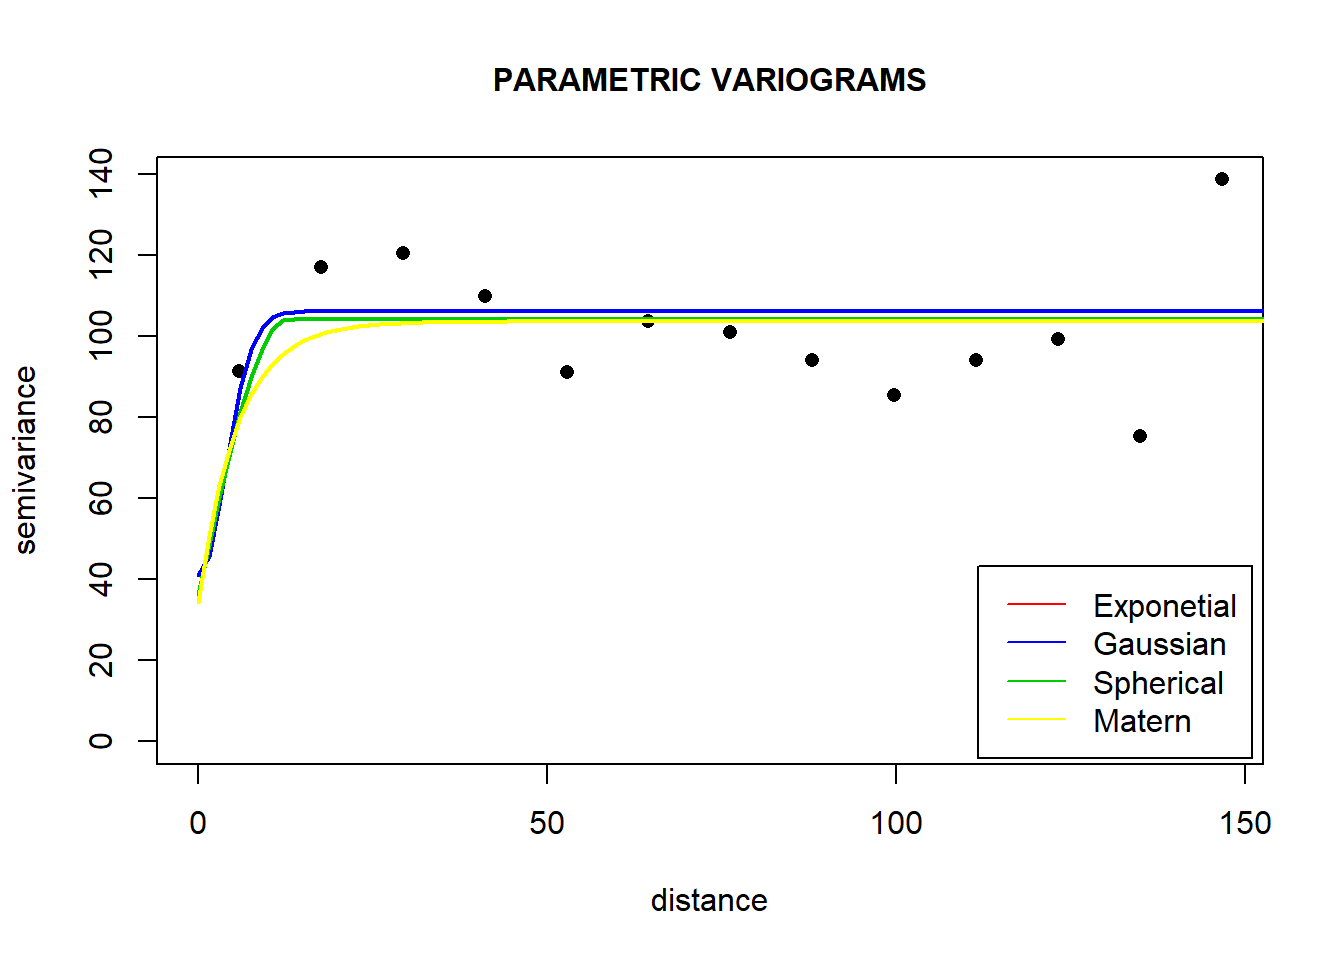
\includegraphics[width=0.7\linewidth]{Assignment_1_FINALE_files/figure-latex/unnamed-chunk-37-1} \end{center}

\hypertarget{gaussian-1}{%
\paragraph{Gaussian}\label{gaussian-1}}

Let's try using the gaussian model to do our prediction step:

\begin{verbatim}
## krige.conv: model with constant mean
## krige.conv: Kriging performed using global neighbourhood
\end{verbatim}

\begin{center}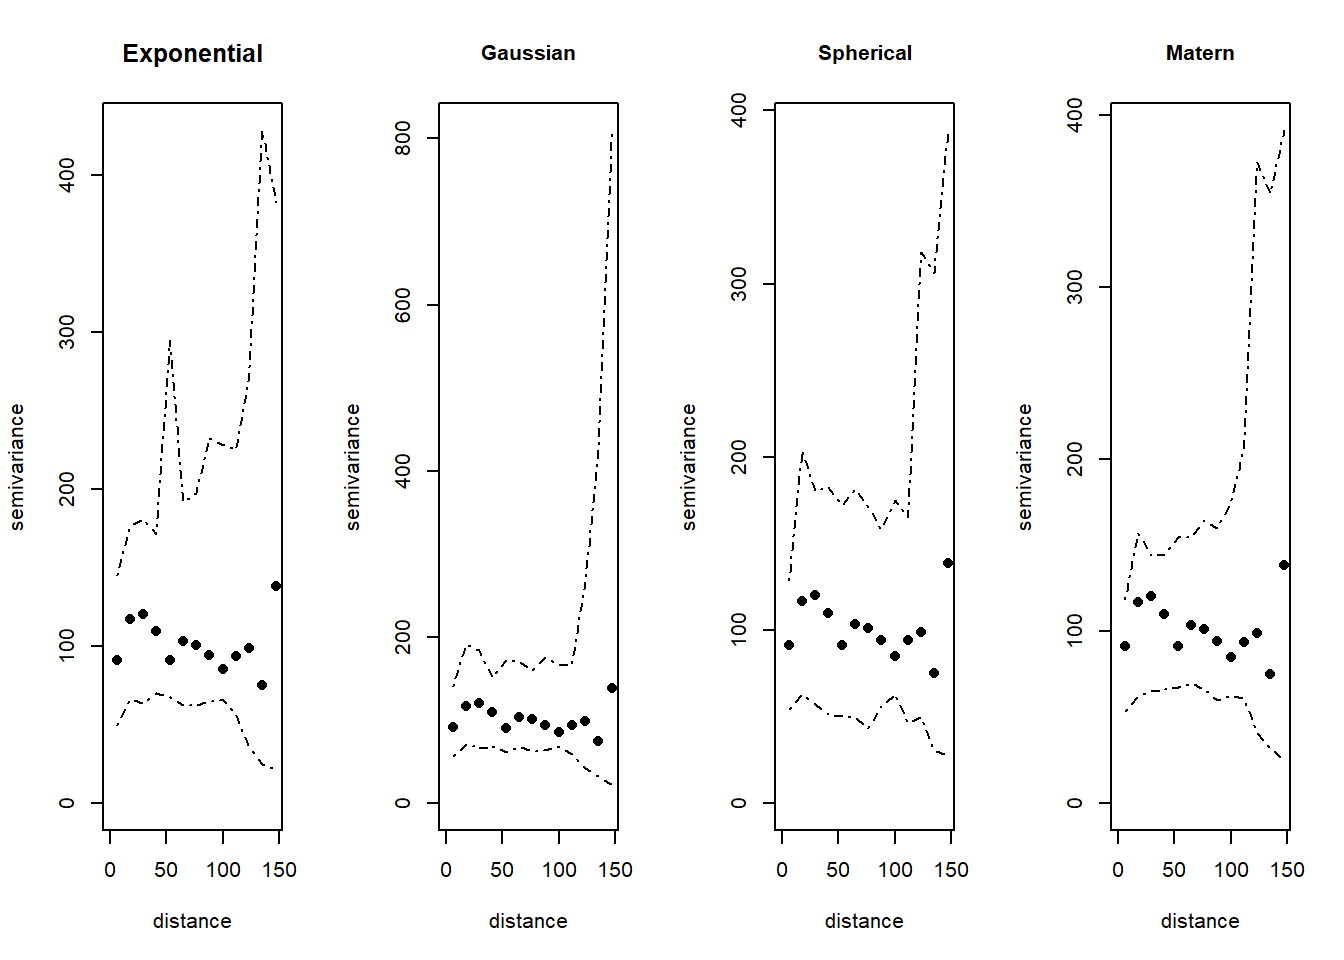
\includegraphics[width=0.7\linewidth]{Assignment_1_FINALE_files/figure-latex/unnamed-chunk-38-1} \end{center}

\begin{center}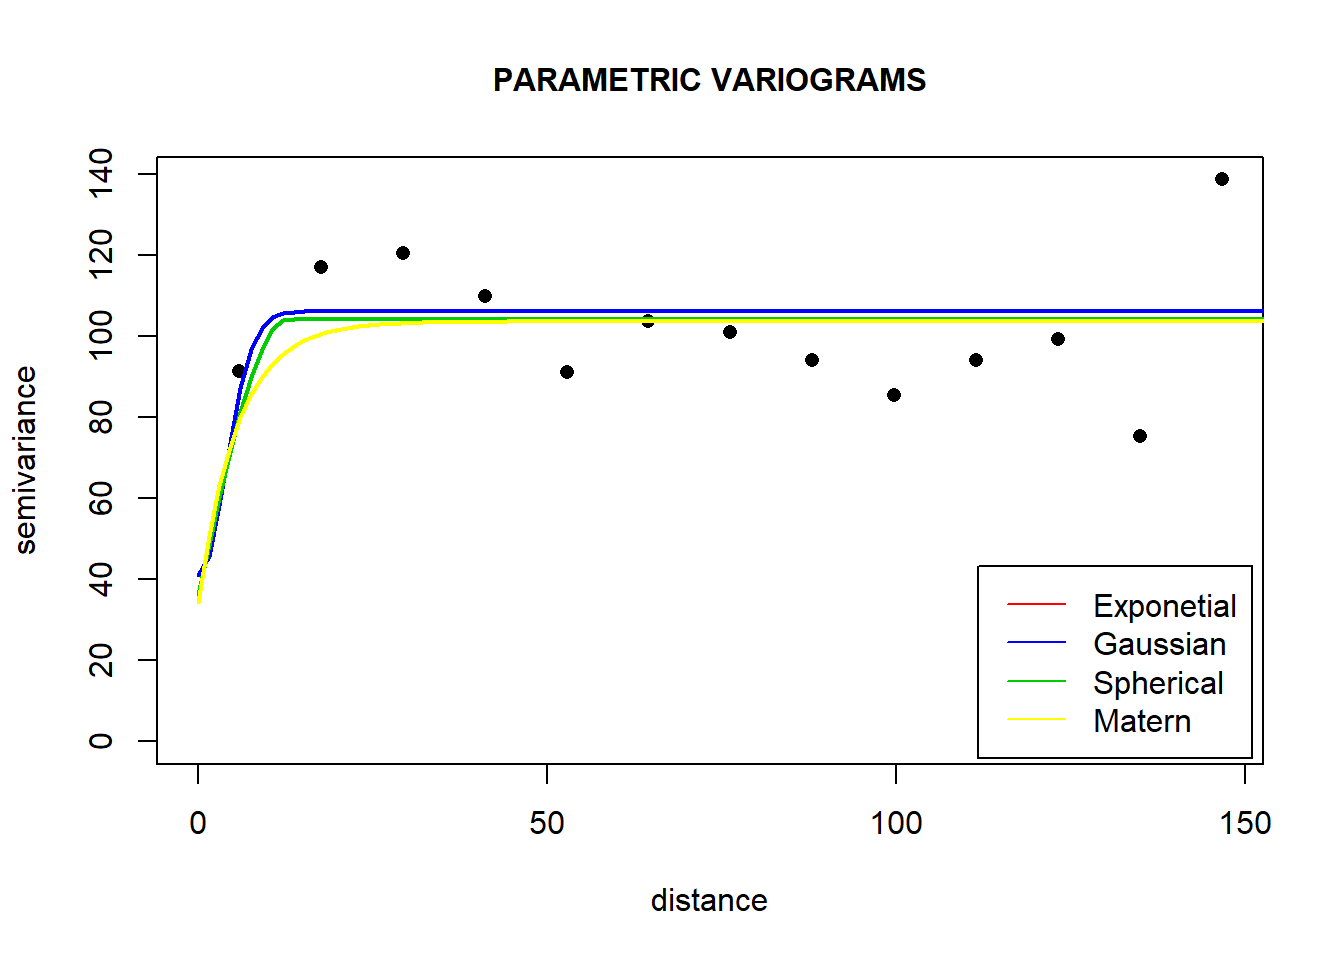
\includegraphics[width=0.7\linewidth]{Assignment_1_FINALE_files/figure-latex/unnamed-chunk-39-1} \end{center}

\begin{center}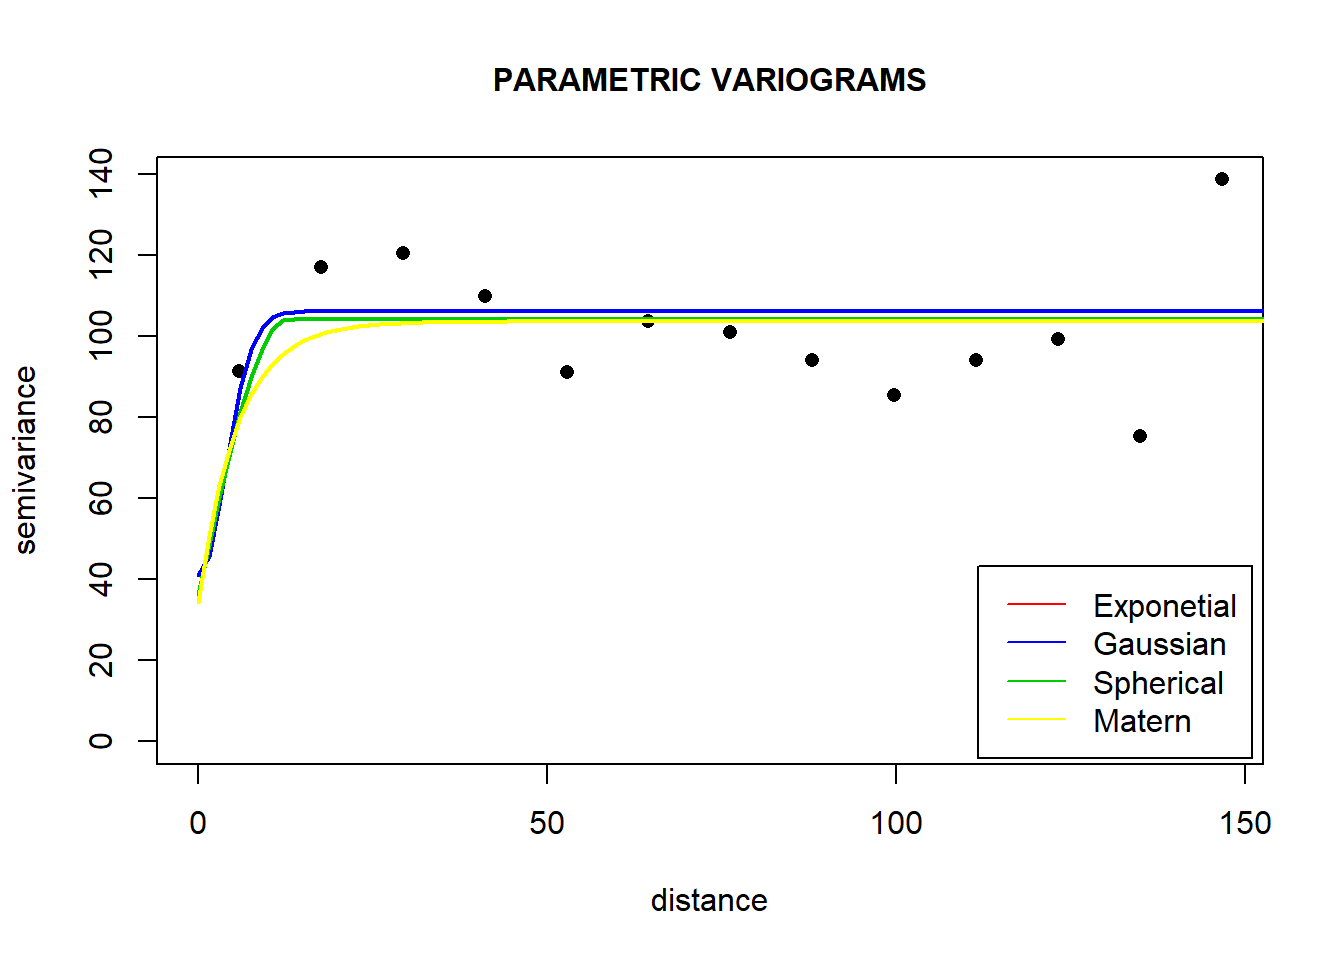
\includegraphics[width=0.7\linewidth]{Assignment_1_FINALE_files/figure-latex/unnamed-chunk-40-1} \end{center}

\begin{verbatim}
## xvalid: number of data locations       = 148
## xvalid: number of validation locations = 148
## xvalid: performing cross-validation at location ... 1, 2, 3, 4, 5, 6, 7, 8, 9, 10, 11, 12, 13, 14, 15, 16, 17, 18, 19, 20, 21, 22, 23, 24, 25, 26, 27, 28, 29, 30, 31, 32, 33, 34, 35, 36, 37, 38, 39, 40, 41, 42, 43, 44, 45, 46, 47, 48, 49, 50, 51, 52, 53, 54, 55, 56, 57, 58, 59, 60, 61, 62, 63, 64, 65, 66, 67, 68, 69, 70, 71, 72, 73, 74, 75, 76, 77, 78, 79, 80, 81, 82, 83, 84, 85, 86, 87, 88, 89, 90, 91, 92, 93, 94, 95, 96, 97, 98, 99, 100, 101, 102, 103, 104, 105, 106, 107, 108, 109, 110, 111, 112, 113, 114, 115, 116, 117, 118, 119, 120, 121, 122, 123, 124, 125, 126, 127, 128, 129, 130, 131, 132, 133, 134, 135, 136, 137, 138, 139, 140, 141, 142, 143, 144, 145, 146, 147, 148, 
## xvalid: end of cross-validation
\end{verbatim}

\begin{verbatim}
## [1] "data"      "predicted" "krige.var" "error"     "std.error" "prob"
\end{verbatim}

\begin{verbatim}
##   index      value
## 1   VC1 0.03902553
## 2   VC2 1.03294158
## 3   VC3 8.68269629
\end{verbatim}

\hypertarget{matern-1}{%
\paragraph{Matern}\label{matern-1}}

\begin{verbatim}
## krige.conv: model with constant mean
## krige.conv: Kriging performed using global neighbourhood
\end{verbatim}

\begin{center}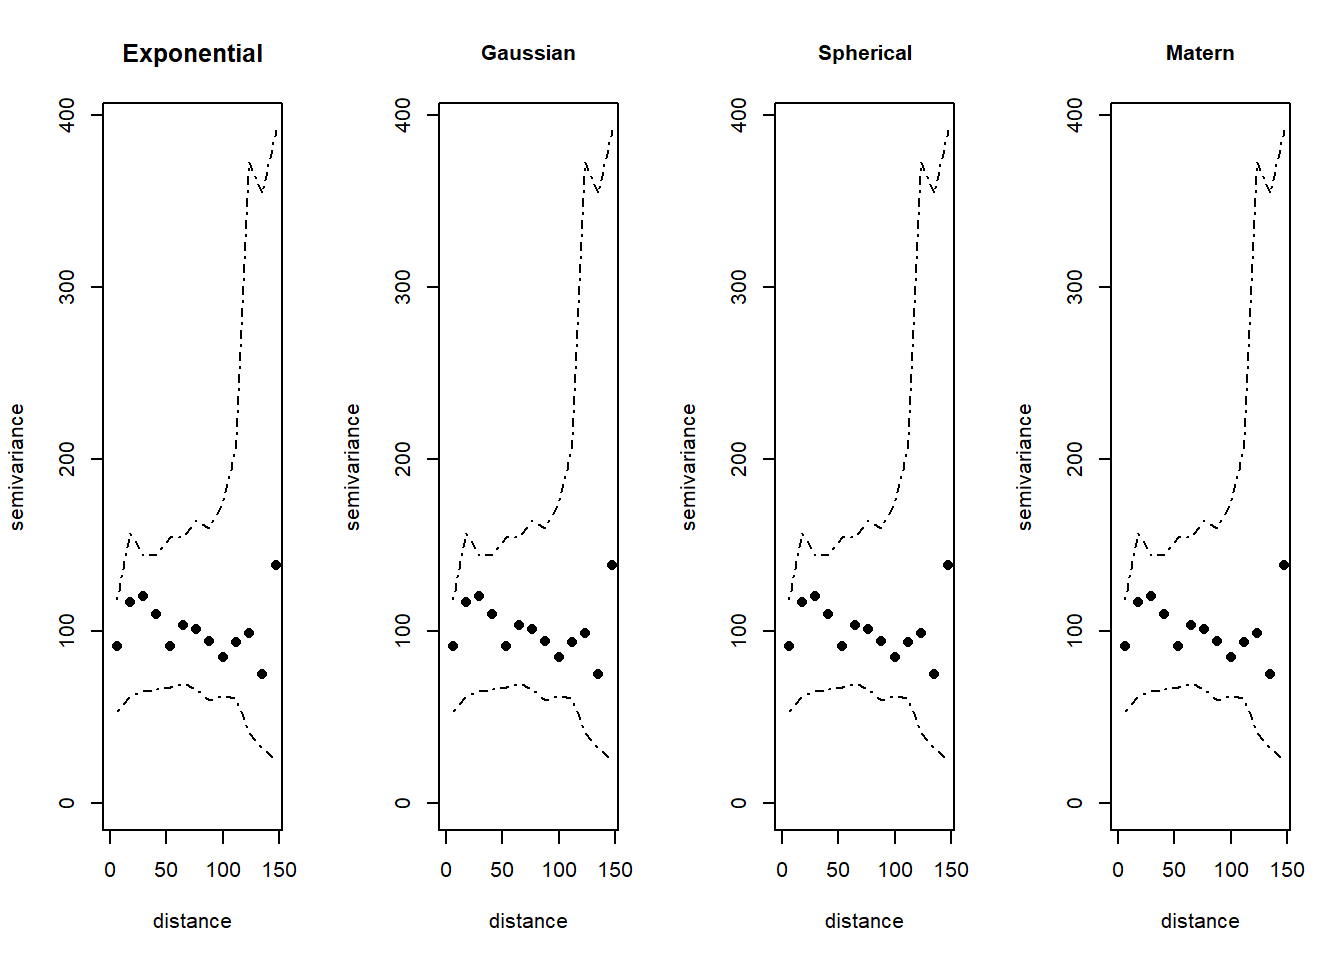
\includegraphics[width=0.7\linewidth]{Assignment_1_FINALE_files/figure-latex/unnamed-chunk-43-1} \end{center}

\begin{center}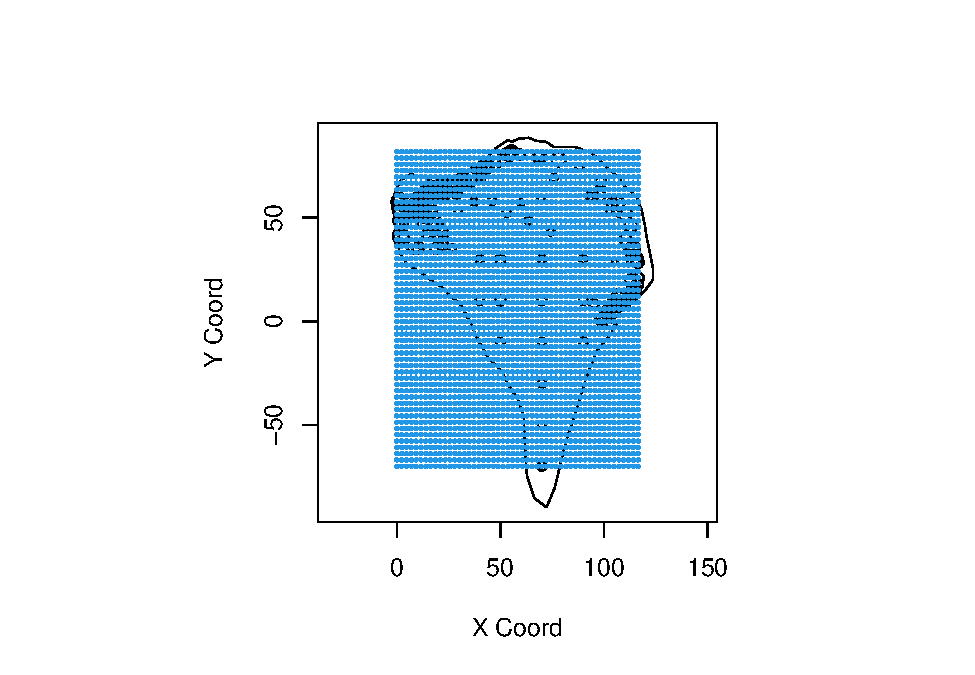
\includegraphics[width=0.7\linewidth]{Assignment_1_FINALE_files/figure-latex/unnamed-chunk-44-1} \end{center}

\begin{center}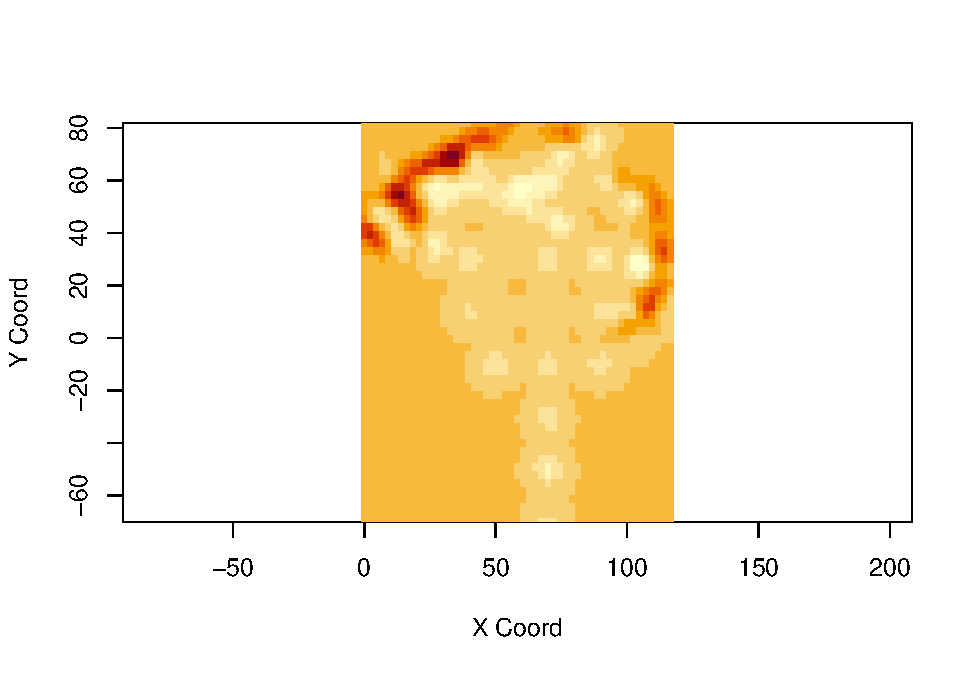
\includegraphics[width=0.7\linewidth]{Assignment_1_FINALE_files/figure-latex/unnamed-chunk-45-1} \end{center}

\begin{verbatim}
## xvalid: number of data locations       = 148
## xvalid: number of validation locations = 148
## xvalid: performing cross-validation at location ... 1, 2, 3, 4, 5, 6, 7, 8, 9, 10, 11, 12, 13, 14, 15, 16, 17, 18, 19, 20, 21, 22, 23, 24, 25, 26, 27, 28, 29, 30, 31, 32, 33, 34, 35, 36, 37, 38, 39, 40, 41, 42, 43, 44, 45, 46, 47, 48, 49, 50, 51, 52, 53, 54, 55, 56, 57, 58, 59, 60, 61, 62, 63, 64, 65, 66, 67, 68, 69, 70, 71, 72, 73, 74, 75, 76, 77, 78, 79, 80, 81, 82, 83, 84, 85, 86, 87, 88, 89, 90, 91, 92, 93, 94, 95, 96, 97, 98, 99, 100, 101, 102, 103, 104, 105, 106, 107, 108, 109, 110, 111, 112, 113, 114, 115, 116, 117, 118, 119, 120, 121, 122, 123, 124, 125, 126, 127, 128, 129, 130, 131, 132, 133, 134, 135, 136, 137, 138, 139, 140, 141, 142, 143, 144, 145, 146, 147, 148, 
## xvalid: end of cross-validation
\end{verbatim}

\begin{verbatim}
##   index      value
## 1   VC1 0.03877583
## 2   VC2 1.03249363
## 3   VC3 8.67909161
\end{verbatim}

\end{document}
